% !TEX TS-program = lualatex
\documentclass[russian,aspectratio=169,14pt,dvipsnames]{beamer}
\usepackage[utf8]{inputenc}
\usepackage[T2A]{fontenc}
\usepackage{listings}
\usepackage{tikz}
\usepackage{amsmath}
\usepackage[]{hyperref}
\usepackage{ulem}

\usetikzlibrary{arrows,shapes,calc}

% Allows to disable rendering of all the slides
\let\ifrender\iftrue
%\let\ifrender\iffalse

\hypersetup{
%    pdfauthor={Vladimir Sitnikov},
%    pdftitle={JMM},
    pdfsubject={Final fields semantics in java memory model},
    pdfkeywords={jmm, final, freeze, dereference chain, memory chain, happens before},
    bookmarksnumbered=true,
    bookmarksopen=true,
    bookmarksopenlevel=1,
    colorlinks=true,
    pdfstartview=Fit,
    pdfpagemode=UseOutlines,
    pdfpagelayout=SinglePage
}

\beamertemplatenavigationsymbolsempty
\setbeamertemplate{footline}[page number]

\definecolor{mygreen}{rgb}{0,0.4,0}
\definecolor{myid}{rgb}{0.1,0.1,0.1}
\lstdefinestyle{Java}{language=java,
        numbers=none,stepnumber=1,numberstyle=\small\ttfamily,
        numbersep=5pt,extendedchars=true,
        commentstyle=\color{mygreen}\ttfamily,
        stringstyle=\color{magenta},
        keywordstyle=\color{violet}\bfseries,
        ndkeywordstyle=\color{yellow}\bfseries,
        identifierstyle=\color{myid},
        basicstyle=\small\ttfamily,
        escapechar=~,
        frame=none,
        lineskip=5pt,
        tabsize=2
}

\lstset{breakatwhitespace=false,
        language=Java,
        style=Java,
}

% Colorbrewer2, 4-class Pastel1
\definecolor{c1}{RGB}{251,180,174}
\definecolor{c2}{RGB}{179,205,227}
\definecolor{c3}{RGB}{204,235,197}
\definecolor{c4}{RGB}{222,203,228}

\definecolor{hbcolor}{named}{c1}
\definecolor{mccolor}{named}{c2}
\definecolor{drcolor}{named}{c3}
\definecolor{hbscolor}{named}{c4}

\tikzstyle{labelfont} = [font=\ttfamily\small\bfseries]
\tikzstyle{na} = [anchor=base,baseline,rectangle,draw,labelfont]
\tikzstyle{main node} = [na,fill=black!20]
\tikzstyle{target node} = [na,fill=Goldenrod!20]
\tikzstyle{hb label} = [fill=hbcolor,labelfont]
\tikzstyle{mc label} = [fill=mccolor,labelfont]
\tikzstyle{dr label} = [fill=drcolor,labelfont]
\tikzstyle{hbs label} = [fill=hbscolor,labelfont]
\tikzstyle{edge style} = [thick,line width=2,labelfont,text=black]
\tikzstyle{hb edge} = [hbcolor,edge style,every node/.style={hb label}]
\tikzstyle{mc edge} = [mccolor,edge style,every node/.style={mc label}]
\tikzstyle{dr edge} = [drcolor,edge style,every node/.style={dr label}]
\tikzstyle{hbs edge} = [hbscolor,edge style,every node/.style={hbs label}]
\tikzstyle{maybe} = [dashed]

\tikzset{alt/.code args={#1#2#3}{%
\if\relax#1\relax\pgfkeysalso{#3}\else\alt<#1>{\pgfkeysalso{#2}}{\pgfkeysalso{#3}}\fi%
}}	

\newcommand{\newarrow}[3]{
\newcommand{#1}{\xrightarrow{\fcolorbox{#3}{#3}{\scriptsize #2}}}
}

\newarrow{\hb}{hb}{hbcolor}
\newarrow{\mc}{mc}{mccolor}
\newarrow{\dr}{dr}{drcolor}
\newarrow{\hbs}{$hb^*$}{hbscolor}

\newcommand{\colbox}[3]{
\newcommand{#1}{\fcolorbox{#3}{#3}{#2}}
}

\colbox{\hbbox}{hb}{hbcolor}
\colbox{\mcbox}{mc}{mccolor}
\colbox{\drbox}{dr}{drcolor}
\colbox{\hbsbox}{$hb^*$}{hbscolor}

\newcommand{\result}{\lstinline!result!}

\newcommand<>\nd[2][]{%
\ifx\relax#3\relax\tikz[na]\node[alt={#1}{target node}{main node}] {#2};%
\else\tikz[na]\node#3[alt={#1}{target node}{main node}] (#2) {#2};\fi%
}

\newcommand<>{\redcross}[1]{
\draw#2[red, line width=0.3mm]
    (#1.south west) -- (#1.north east)
    (#1.south east) -- (#1.north west);%
}

\renewcommand<>{\sout}[1]{
  \alt#2{\beameroriginal{\sout}{#1}}{#1}
}

\newcommand<>\dimunless[1]{\alt#2{\textcolor{black}{#1}}{\textcolor{black!20}{#1}}}

\newcommand{\hbsprogresss}[9]{%
\begin{tikzpicture}[overlay]%
\node [anchor=north east, inner sep=10pt] at (current page.north east){%
$\dimunless<#1>{w}~\dimunless<#2>{\xrightarrow{hb}}~\dimunless<#3>{f}~\dimunless<#4>{\xrightarrow{hb}}~\dimunless<#5>{a}~\dimunless<#6>{\xrightarrow{mc}}~\dimunless<#7>{r1}~\dimunless<#8>{\xrightarrow{dr}}~\dimunless<#9>{r2}$%
};%
\end{tikzpicture}%
}

\newcommand{\hbsprogress}[4]{\hbsprogresss{#1}{#1}{#1}{#2}{#2}{#3}{#3}{#4}{#4}}

\newcommand\vskiptitle{\vglue0.25cm}
\newcommand\vskipfill{\vglue0pt plus 1filll}

\tikzstyle{every picture}+=[remember picture]

%\setcounter{tocdepth}{1}
\ifrender
\AtBeginSection[]
{
  \begin{frame}<beamer>
    \setcounter{tocdepth}{1}
    \tableofcontents[currentsection]
    \setcounter{tocdepth}{5}
  \end{frame}
}
\fi

\begin{document}
\title[JMM: semantics of final fields]{Semantics of final fields in java}
\author{Vladimir Sitnikov, Valentin Kovalenko\newline{\footnotesize sitnikov@netcracker.com, @VladimirSitnikv}}
\institute[NetCracker Tech]{\small NetCracker}
\date{\small September 2014}

\ifrender
\begin{frame}[plain,noframenumbering]
  \titlepage
\end{frame}
\fi


\section{Введение}

\ifrender
\begin{frame}
\Huge Зачем нам JMM?
\end{frame}
\fi

% ---------------------------------------
% Вступительная загадка
%
\ifrender
% lstlisting cannot be placed inside \only :(
\defverbatim[colored]\lstIntOne{%
\begin{lstlisting}
int x = 1;
\end{lstlisting}
}
\defverbatim[colored]\lstFinalIntOne{%
\begin{lstlisting}
final int x = 1;
\end{lstlisting}}

\subsection{Загадка}
\begin{frame}[fragile]{Код-загадка}
\begin{center}%
\begin{minipage}[3]{0.5\textwidth}%
\only<1-2>{\lstIntOne}%
\only<3-4>{\lstFinalIntOne}%
\begin{lstlisting}[]
public int neverTryThisAtHome() {
  int i = this.x; // it is 1, isn't it?
  this.setX(2); // just updates x to 2
  return this.x - i; // 2 - 1 == ...?
}
\end{lstlisting}%
\end{minipage}%
\end{center}%
\only<1>{Какие значения могут вернуться? 1? 0? -1?}
\only<2>{Да, тут вернётся 1}
\only<3>{А теперь добавим \sout{ножек} \lstinline!final!}
\only<4>{Спецификация разрешает все варианты: 1, 0, и даже -1! (см. пример 17.5.3-1)}
\vskipfill
\end{frame}
\fi


\ifrender
\begin{frame}
\Huge Why \lstinline[basicstyle=\Huge\ttfamily]!final! is required in JMM?
\end{frame}
\fi

% ---------------------------------------
% java 1.4 & String security
%
\ifrender

\newcommand{\tikzref}[2]{% to define an anchor
  \tikz[remember picture]{%
    \coordinate (#1) at (#2);%
 }%
}

\defverbatim[colored]\lstHackStringThread{%
\begin{minipage}[t]{.5\textwidth}%
\begin{lstlisting}[title=HackThread]
GLOBAL =
  "/tmp/etc/passwd"
  .~\tikzref{sub}{0,0.5ex}~substring(4);
\end{lstlisting}%
\end{minipage}%
}

\defverbatim[colored]\lstHandleString{%
\begin{lstlisting}
String s = ...
if (checkAccess(s)) {
  return readFile(s);
}
\end{lstlisting}%
}

\defverbatim[colored]\lstGetAndHandleString{%
\begin{lstlisting}
String s = GLOBAL;
if (checkAccess(s~\tikzref{s1}{0,1ex}~)) {
  return readFile(s~\tikzref{s2}{0,0}~);
}
\end{lstlisting}
}

\subsection{Final и безопасность}
\begin{frame}[fragile]
\frametitle{\alt<1,8>{Без}{\sout{Без}}опасность String \only<2-7>{в java 1.4}\only<8>{в java 1.5+}}
\vskiptitle
\begin{minipage}[t]{.5\textwidth}%
\alt<1-2>{\begin{minipage}[t]{.5\textwidth}\lstHandleString\end{minipage}%
}{\begin{minipage}[t]{.5\textwidth}\lstGetAndHandleString\end{minipage}%
}%
\end{minipage}%
\only<3->{\begin{minipage}[t]{.5\textwidth}\lstHackStringThread\end{minipage}%
}%
\vskipfill
% Стрелочки между tikz-якорями
\begin{tikzpicture}[overlay]
  \path[hb edge,->]<5-7> (sub) edge [out=120,in=45,looseness=1] node {race} (s1);
  \path[hb edge,->]<5-7> (sub) edge [out=-130,in=-60,looseness=1] node {race} (s2);
  \path[hbs edge,->]<8> (sub) edge [out=120,in=45,looseness=1] node {hb} (s1);
  \path[hbs edge,->]<8> (sub) edge [out=-130,in=-60,looseness=1] node {hb} (s2);
\end{tikzpicture}
\only<1>{Правильно ли проверяются права на доступ к файлу?}%
\only<2>{Ответ зависит от версии, и в java 1.4 возможны проблемы}
\only<3>{Например: HackThread выполняет \lstinline!.substring(4)! и коварно передаёт его в поток, читающий файлы}%
\only<4>{В java 1.4 substring-строка ссылается на тот же массив символов, и всё опреледяется полями \lstinline!String##offset! и \lstinline!String##size!}%
\only<5>{Синхронизации между потоками нет, поэтому читатель может увидеть недоинициализированный объект-строку}%
\only<6-7>{\lstinline!checkAccess! может увидеть \lstinline!"/tmp/etc/passwd"!,
а \lstinline!readFile! уже \lstinline!"/etc/passwd"!%
\uncover<7>{\parДаже синхронизация на \lstinline!s! и \lstinline!volatile! не спасут!}
}%
\only<8>{В java 1.5+ \lstinline!final! защищает от недосозданных объектов и HackTread}%
\note{Синхронизация и volatile по string не поможет, т.к. HackThread не будет их использовать}%
\vskipfill
\end{frame}
\fi


\ifrender
\begin{frame}
\Huge Немного теории
\end{frame}
\fi

\ifrender
\subsection{Program order}
\begin{frame}{Program order}
\begin{itemize}[<+->]
\item Program order is a total order among inter-thread actions of each thread in source code order
\item Compiler is forbidden to reorder/alter/ignore operations if observable behavior violates program order
\item It does not mean the program is executed in program order
\item For instance: program order is not defined for operations on local variables
\end{itemize}
\end{frame}
\fi

\ifrender
\subsection{Частичный порядок (partial order)}
\begin{frame}{Частичный порядок (partial order)}
\begin{itemize}[<+->]
\item В главе 17 JLS 8 раз упоминается слово "partial order"
\item Частичным порядком $\hb$ является бинарное отношение, которое:
\begin{itemize}
\item Рефлексивно: для любого элемента $x$ выполняется $x \hb x$
\item Антисимметрично: если $x \hb y$ и $y \hb x$, то $x$ и $y$ это одно и то же
\item Транзитивно: если $x \hb y$ и $y \hb z$, то $x \hb z$
\end{itemize}
\end{itemize}
\end{frame}
\fi

\ifrender
\subsection{Happens-before}
\begin{frame}{Happens-before}
\begin{itemize}[<+->]
\item Основной принцип JMM: рассмотрим все возможные выполнения и откинем "неправильные"
\item Happens-before это частичный порядок, который должен соблюдаться
\item Запрещено видеть "будущие" записи ($r \hb w$)
\item И те, которые были перетёрлись в {\hbbox} порядке: $w1 \hb w2 \hb r$
\item И те, которые запрещены просто так: 17.4.8 executions and causality requirements
\end{itemize}
\end{frame}
\fi


% ---------------------------------------
% HB*
%
\ifrender
\subsection{HB$^*$}
\begin{frame}[fragile]{Семантика final полей одним слайдом}
\vskip1.5cm
\scalebox{1.5}{$w \hb f \hb a \mc r1 \dr r2 \Rightarrow w \hbs r2$}
\vskip1.3cm
\only<1-2>{%
\begin{itemize}[<+->]
\item $w$ и $r2$ -- интересующие нас нас запись и чтение
\item $f$ -- заморозка \lstinline!final! поля, которое читается в $r1$
\end{itemize}
}%
\only<3-4>{%
\begin{itemize}[<+(2)->]
\item Если единственный путь от записи к чтению идёт через все эти стрелочки, то мы не можем увидеть более ранние записи
\item Если путей больше одного -- как повезёт
\end{itemize}
}%
\vskipfill
\end{frame}
\fi


% ---------------------------------------
% Freeze action. Definition
%
\ifrender
\tikzstyle{large arrow} = [single arrow,fill=black!20]
\subsection{Freeze action}
\begin{frame}[fragile]{Freeze action}%
\hbsprogresss{0}{0}{1-}{0}{0}{0}{0}{0}{0}%
\hbox to \hsize{\hfil%
\begin{tikzpicture}[auto]%
  \node at (0,0) {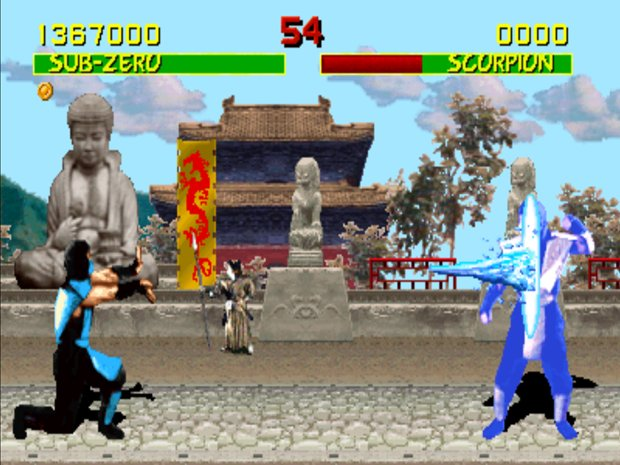
\includegraphics[trim=0 0 0 180,clip,width=0.85\textwidth]{freeze_action.jpg}};
  \node<2-> [large arrow,anchor=mid east] at (3cm, 0.8cm) {\LARGE Freeze action};
  \uncover<3->{\node [large arrow,anchor=mid west,shape border rotate=180] at (5.1cm, -0.5cm) {\LARGE Field};}
\end{tikzpicture}%
\hfil}%
\\\uncover<3>{Freezes of a \lstinline!final! field occur both at the end of the constructor, and immediately after each modification}%
\end{frame}
\fi


% ---------------------------------------
% Dereference chain. Пример возникновения
%
\ifrender
\subsection{Dereference chain}
\begin{frame}[fragile]{Dereference chain: что это?}
\hbsprogresss{0}{0}{0}{0}{0}{0}{0}{1-}{0}%
\vskiptitle
\begin{center}
\begin{minipage}[3]{.5\linewidth}
	\begin{lstlisting}
T local = GLOBAL; ~\nd<1->{r1}~

int localX = local.x; ~\nd<1->[1-]{r2}~
	\end{lstlisting}
\end{minipage}
\end{center}

\vskipfill

% Стрелочки между tikz-якорями
\begin{tikzpicture}[overlay]
  \path[dr edge,->]<4-> (r1) edge [bend right, out = 90, in = 90, looseness = 2] node {dr} (r2);
\end{tikzpicture}%

\begin{itemize}[<+->]
\item \nd[1-]{r2} читает поле объекта
\item Поток не создавал объект
\item Значит, где-то мы должны были читать адрес этого объекта
\item Это называется $r1 \dr r2$
\end{itemize}

\vskipfill

\end{frame}
\fi

% ---------------------------------------
% Dereference chain. Между потоками не возникает
%
\ifrender
\begin{frame}[fragile]{Dereference chain между потоками}
\vskiptitle
\begin{minipage}[t]{.49\textwidth}
	\begin{lstlisting}[title=Thread 1]
T localA = new T(); ~\nd<2->[2,3]{a}~
GLOBAL = localA;
	\end{lstlisting}
\end{minipage}
\begin{minipage}[t]{.49\textwidth}
	\begin{lstlisting}[title=Thread 2]
T localB = GLOBAL; ~\nd<1->[1]{r1}~
if (localB != null) {
  int localX = localB.x; ~\nd<1->[1-]{r2}~
}
\end{lstlisting}
\end{minipage}

\vskipfill

\begin{tikzpicture}[overlay]
  \path[dr edge,->]<1-> (r1) edge [bend right, out = 90, in = 90, looseness = 2] node {dr} (r2);
  \path[dr edge,maybe,->]<2-> (a) edge [bend right, out = 270, in = 270, looseness = 0.8] node (drq) {dr?} (r2);
  \redcross<3->{drq}
\end{tikzpicture}

\begin{center}
\only<1>{$r1 \dr r2$ (читаем поле несозданного нами объекта)}%
\only<2>{Есть ли $a \dr r2$?}%
\only<3>{Между потоками {\drbox} не возникает!}%
\end{center}

\vskipfill

\end{frame}
\fi

% ---------------------------------------
% Dereference chain. Контрольный выстрел
%
\ifrender
\begin{frame}[fragile]{Dereference chain: контрольный выстрел}
\hbsprogresss{0}{0}{0}{0}{0}{0}{0}{1-}{0}%
\vskiptitle
\begin{center}
\begin{minipage}{.5\linewidth}
	\begin{lstlisting}
T local = GLOBAL; ~\nd<1->[2]{ra}~

local = GLOBAL; ~\nd<1->[2]{rb}~

int localX = local.x; ~\nd<1->{r2}~
	\end{lstlisting}
\end{minipage}%
\end{center}%

\vskipfill

\begin{tikzpicture}[overlay]%
  \path[dr edge,maybe,->]<2-> (ra) edge [bend right, out = 90, in = 90, looseness = 2] node {dr?} (r2);
  \path[dr edge,maybe,->]<2-> (rb) edge [bend right, out = 90, in = 90, looseness = 1] node {dr?} (r2);
\end{tikzpicture}%

\begin{center}
\only<1>{Есть ли здесь \drbox?}%
\only<2>{Один из $ra \dr r2$ или $rb \dr r2$ точно должен быть, но точнее сказать невозможно}%
\end{center}

\vskipfill

\end{frame}
\fi


% ---------------------------------------
% Memory chain. Definition.
%
\ifrender
\subsection{Memory chain}
\begin{frame}[fragile]{Memory chain: what is that?}
\hbsprogresss{0}{0}{0}{0}{0}{1-}{0}{0}{0}%
\vskip0.25cm
\begin{minipage}[t]{.33\textwidth}
	\begin{lstlisting}[title=Thread 1]
T o = new T();
GL = o; ~\nd<1->[1,6]{w1}~
	\end{lstlisting}
\end{minipage}%
\begin{minipage}[t]{.33\textwidth}
	\begin{lstlisting}[title=Thread 2]
T o = GL; ~\nd<1->[1,2]{r1}~
GL2 = o; ~\nd<2->[2,3]{w2}~
\end{lstlisting}
\end{minipage}%
\begin{minipage}[t]{.33\textwidth}
	\begin{lstlisting}[title=Thread 3]
T o = GL2; ~\nd<3->[3-5]{r3}~
int r = o.x; ~\nd<4->[4-6]{r4}~
\end{lstlisting}
\end{minipage}

\vskipfill

% Стрелочки между tikz-якорями
\begin{tikzpicture}[overlay]
  \path[mc edge,->]<1-> (w1) edge [bend left=30] node {mc} (r1);
  \path[mc edge,->]<2-> (r1) edge [out=0, in=-45, looseness=3] node {mc} (w2);
  \path[mc edge,->]<3-> (w2) edge [bend left=30] node {mc} (r3);
  \path[dr edge,->]<4-> (r3) edge [out=45, in=45, looseness=2.5] node {dr} (r4);
  \path[mc edge,->]<5-> (r3) edge [out=235, in=235, looseness=2.5] node {mc} (r4);
  \path[mc edge,->]<6-> (w1) edge [out=-90, in=-90, looseness=0.4] node {mc} (r4);
\end{tikzpicture}

\begin{center}
\only<1>{If a read sees write, then $w1 \mc r1$}%
\only<2>{If a thread writes the address of an object that was initialized in another thread, then $r1 \mc w2$}%
\only<3>{\nd[3]{r3} sees \nd[3]{w2} $\Rightarrow w2 \mc r3$}%
\only<4,5>{$r3 \dr r4$ (read of a object's field) \uncover<5>{$\Rightarrow r3 \mc r4$}}%
\only<6>{{\mcbox} is transitive (it is a partial order) $\Rightarrow w1 \mc r4$}%
\end{center}

\vskipfill

\end{frame}
\fi


\section{Примеры}
% ---------------------------------------
% Disclaimer
%
\ifrender
%\subsection{Disclaimer}
\begin{frame}[fragile]{Disclaimer}%
\begin{itemize}[<+->]
\item Все примеры опасно синхронизированы (иначе зачем мы собрались?)
\item Случаи чтения null не рассматриваем (даже если они возможны)
\item При составлении слайдов пострадал не один мозг
\end{itemize}
\end{frame}
\fi


% ---------------------------------------
% Example 1 "trivial final field"
%
\ifrender
\subsection{Trivial final (1)}
\begin{frame}[fragile]{Trivial final (1)}
\hbsprogress{2-}{2-}{6-}{7-}%
\vskiptitle
\begin{minipage}{0.5\textwidth}
	\begin{lstlisting}[title=Thread 1]
T l = new T() {{
  fx = 42; ~\nd<1->[1,2,4,8,9]{w}~
}}; ~\nd<2->[2]{f}~
GLOBAL = l; ~\nd<2->[2,3,6]{a}~
	\end{lstlisting}
\end{minipage}%
\begin{minipage}{0.5\textwidth}
	\begin{lstlisting}[title=Thread 2]
T o = GLOBAL; ~\nd<3-6>[3,4,5]{r0}~
if (o != null) {
  int result = o.fx; ~\nd<4->[4,5,6,7]{r1}~ ~\nd<1,7->[1,7,8,9]{r2}~
}
	\end{lstlisting}
\end{minipage}

\vskipfill

\begin{tikzpicture}[overlay]
  \path[hb edge,->]<2-> (w) edge [out=120, in=110, looseness=2.5] node {hb} (f);
  \path[hb edge,->]<2-> (f) edge [bend left=15] node {hb} (a);
  \path[mc edge,->]<3-6> (a) edge [bend left=40, in=140] node {mc} (r0);
  \path[dr edge,->]<4-5> (r0) edge [bend right, out = 270, in = 270, looseness = 2] node {dr} (r1);
  \path[mc edge,->]<5,6> (r0) edge [bend left=20] node {mc} (r1);
  \path[mc edge,->]<6> (a) edge [bend left=70, in=90, looseness=1.2] node {mc} (r1);
  \path[mc edge,->]<7-> (a) edge [bend left=45, in=135] node {mc} (r1);
  \path[dr edge,->]<7-> (r1) edge [out=-90, in=-90, looseness = 1.5] node {dr} (r2);
  \path[hbs edge,->]<8-> (w) edge [bend right, out = 45, in = 110, looseness = 1.0] node {hb*} (r2);
\end{tikzpicture}

\begin{center}
\only<1>{Can \result~become $0$?}%
\only<2>{Actions in a thread form happens-before:\\ $w \hb f$, $f \hb a$}%
\only<3>{\nd[3]{r0} sees write \nd[3]{a}:\\ $a \mc r0$}%
\only<4>{Thread 2 did not create the object, \nd[4]{r1} reads its field, and \nd[4]{r} is the only read of the address, thus we have dereference chain:\\ $r0 \dr r1$}%
\only<5>{$r0 \dr r1 \Rightarrow r0 \mc r1$}%
\only<6>{$a \mc r1$ ({\mcbox} is transitive)}%
\only<7>{Let's pick $r2 = r1$, then $r1 \dr r2$ ({\drbox} is reflexive)}%
\only<8>{Here all the requirements for $HB^*$: \\$w \hb f \hb a \mc r1 \dr r2 \Rightarrow w \hbs r2$}%
\only<9>{$(w \hbs r2) \Rightarrow$ \result~$\in \{42\}$}%
\end{center}

\vskipfill

\end{frame}
\fi

% ---------------------------------------
% Пример 2 "массив внутри final поля"
%
\ifrender
\subsection{Массив внутри final (2)}
\begin{frame}[fragile]{Массив внутри final (2)}
\vskiptitle
\hbsprogress{2-}{2-}{3-}{4-}%
% Сорцы и tikz-якоря
\begin{minipage}{0.5\textwidth}
	\begin{lstlisting}
T l = new T() {{
  int[] u = new int[1];
  u[0] = 42; ~\nd<1->[1,2,5,6]{w}~
  fx = u;
}}; ~\nd<2->[2]{f}~
GLOBAL = l; ~\nd<2->[2,3]{a}~
	\end{lstlisting}
\end{minipage}%
\begin{minipage}{0.5\textwidth}
	\begin{lstlisting}
T o = GLOBAL;
if (o != null) {
  int[] lfx = o.fx; ~\nd<3->[3,4]{r1}~
  int result = lfx[0]; ~\nd<1->[1,4,5,6]{r2}~
}
	\end{lstlisting}
\end{minipage}

\vskipfill

% Стрелочки между tikz-якорями
\begin{tikzpicture}[overlay]
  \path[hb edge,->]<2-> (w) edge [] node {hb} (f);
  \path[hb edge,->]<2-> (f) edge [bend left=15] node {hb} (a);
  \path[mc edge,->]<3-> (a) edge [bend left, looseness=0.7] node {mc} (r1);
  \path[dr edge,->]<4-> (r1) edge [bend right, out = 270, in = 270, looseness = 2.2] node {dr} (r2);
  \path[hbs edge,->]<5-> (w) edge [bend right, out = 90, in = 90, looseness = 0.7] node {hb*} (r2);
\end{tikzpicture}

% Подписи, потихоньку появляющиеся под сорцами
\begin{center}
\only<1>{Возможно ли в \result~получить $0$?}%
\only<2>{Действия в одном потоке образуют happens-before:\\ $w \hb f$, $f \hb a$}%
\only<3>{\nd[3]{r1} видит запись \nd[3]{a} (т.к. простое final поле):\\ $a \mc r1$}%
\only<4>{Поток 2 не создавал массив, $r2$ читает его элемент, $r1$ это единственное чтение адреса массива, поэтому dereference chain:\\ $r1 \dr r2$}%
\only<5>{Нашли всё необходимое для $HB^*$: \\$w \hb f \hb a \mc r1 \dr r2 \Rightarrow w \hbs r2$}%
\only<6>{($w \hbs r2) \Rightarrow$ \result~$\in \{42\}$}%
\end{center}

\vskipfill
\end{frame}
\fi

% ---------------------------------------
% Пример 2.1 "порядок присваивания final"
%
\ifrender
\subsection{Массив наоборот (2.1)}
\begin{frame}[fragile]{Массив наоборот (2.1)}
\vskiptitle
\hbsprogress{2-}{2-}{2-}{2-}%
\begin{minipage}{0.5\textwidth}
	\begin{lstlisting}
T l = new T() {{
  int[] u = new int[1];
  fx = u; // (!)
  u[0] = 42; ~\nd<1->[1,2,3]{w}~
}}; ~\nd<2->{f}~
GLOBAL = l; ~\nd<2->{a}~
	\end{lstlisting}
\end{minipage}%
\begin{minipage}{0.5\textwidth}
	\begin{lstlisting}
T o = GLOBAL;
if (o != null) {
  int[] lfx = o.fx; ~\nd<2->{r1}~
  int result = lfx[0]; ~\nd<2->[2,3]{r2}~
}
	\end{lstlisting}
\end{minipage}

\vskipfill

% Стрелочки между tikz-якорями
\begin{tikzpicture}[overlay]
  \path[hb edge,->]<2-> (w) edge [] node {hb} (f);
  \path[hb edge,->]<2-> (f) edge [bend left=15] node {hb} (a);
  \path[mc edge,->]<2-> (a) edge [bend left, looseness=0.7] node[mc label] {mc} (r1);
  \path[dr edge,->]<2-> (r1) edge [bend right, out = 270, in = 270, looseness = 2.2] node {dr} (r2);
  \path[hbs edge,->]<2-> (w) edge [bend right, out = 90, in = 90, looseness = 0.7] node {hb$^*$} (r2);
\end{tikzpicture}

% Подписи, потихоньку появляющиеся под сорцами
\begin{center}
\only<1>{Возможно ли в \result~получить $0$?}%
\only<2>{Строим {\hbsbox} так же как и в предыдущем случае}%
\only<3>{($w \hbs r2) \Rightarrow$ \result~$\in \{42\}$\\Результат не зависит от порядка записи final полей!}%
\end{center}

\vskipfill

\end{frame}
\fi

% ---------------------------------------
% Пример 3 "утекание this из конструктора"
%
\ifrender
\subsection{Утекание this (3)}
\begin{frame}[fragile]{Утекание this (3)}
\vskiptitle
\hbsprogress{2-}{0}{0}{0}%
% Сорцы и tikz-якоря
\begin{minipage}{0.5\textwidth}
	\begin{lstlisting}[title=Thread 1]
T l = new T() {{
  fx = 42; ~\nd<1->[1,2]{w}~
  GLOBAL = this; ~\nd<2->[2,3,4,5]{a}~
}}; ~\nd<2->[2,3,4]{f}~
	\end{lstlisting}
\end{minipage}%
\begin{minipage}{0.5\textwidth}
	\begin{lstlisting}[title=Thread 2]
T o = GLOBAL;
if (o != null) {
  int result = o.fx; ~\nd<1->[1,5]{r2}~
}
	\end{lstlisting}
\end{minipage}

\vskipfill

% Стрелочки между tikz-якорями
\begin{tikzpicture}[overlay]
  \path[hb edge,->]<2-> (w) edge [out=135, in=135, looseness=1.5] node {hb} (f);
  \path[hb edge,->]<2-> (a) edge [bend left=60] node {hb} (f);
  \path[hb edge,maybe,->]<3-> (f) edge [bend right=5] node (hbq) {hb?} (a);
  \redcross<4->{hbq}
\end{tikzpicture}%

% Подписи, потихоньку появляющиеся под сорцами
\begin{center}
\only<1>{Возможно ли в \result~получить $0$?}%
\only<2>{Действия в одном потоке образуют happens-before:\\ $w \hb f$, $a \hb f$}%
\only<3>{Но нам-то нужно $f \hb a$!}%
\only<4>{Если $a \hb f$ и $f \hb a$, то $a = f$ (антисимметричность {\hbbox})\\Но публикация ссылки это никак не freeze action!}%
\only<5>{Нет \hbsbox, поэтому возможны все варианты: \result~$\in \{0, 42\}$}%
\end{center}
\vskipfill
\end{frame}
\fi

% ---------------------------------------
% Пример 4 "утекание this из конструктора, чтение из другой ссылки"
%
\ifrender
\subsection{Вредительское утекание this (4)}
\begin{frame}[fragile]{Вредительское утекание this (4)}
\vskiptitle
\hbsprogress{2-}{2-}{0}{0}%
% Сорцы и tikz-якоря
\begin{minipage}{0.5\textwidth}
	\begin{lstlisting}[title=Thread 1]
T l = new T() {{
  fx = 42; ~\nd<1->[1,2]{w}~
  GLb = this; ~\nd<2->[6]{b}~
}}; ~\nd<2->[2]{f}~
GLa = l; ~\nd<2->[2,3]{a}~
	\end{lstlisting}
\end{minipage}%
\begin{minipage}{0.5\textwidth}
	\begin{lstlisting}[title=Thread 2]
T u = GLb; ~\nd<4->[4,5,6]{rb}~
T o = GLa; ~\nd<3->[3,4]{ra}~
if (o != null) {
  int result = o.fx; ~\nd<4->[4,5,6]{r1}~ ~\nd<1>[1]{r2}~
}
	\end{lstlisting}
\end{minipage}

\vskipfill

% Стрелочки между tikz-якорями
\begin{tikzpicture}[overlay]
  \path[hb edge,->]<2-> (w) edge [out=120, in=110, looseness=2.5] node {hb} (f);
  \path[hb edge,->]<2-> (f) edge [bend right=80, looseness=1.6] node {hb} (a);
  \path[hb edge,maybe,->]<2-> (f) edge [bend right=10] node (hb-f-b) {hb?} (b);
  \redcross<2->{hb-f-b}
  \path[mc edge,->]<3-> (a) edge [out=27, in=167, looseness=1.3] node {mc} (ra);
  \path[dr edge,maybe,->]<4-> (ra) edge [out=-90, in=235, looseness=1.5] node {dr?} (r1);
  \path[dr edge,maybe,->]<4> (rb) edge [out=0, in=90, looseness=1.5] node {dr?} (r1);
  \path[dr edge,->]<5-> (rb) edge [out=0, in=90, looseness=1.5] node {dr} (r1);
\end{tikzpicture}

% Подписи, потихоньку появляющиеся под сорцами
\begin{center}
\only<1>{Возможно ли в \result~получить $0$?}%
\only<2>{Действия в одном потоке образуют happens-before:\\ $w \hb f$, $f \hb a$}%
\only<3>{Пусть второй поток увидел \lstinline!GLa!, тогда $a \mc ra$!}%
\only<4>{Где-то должно быть \drbox: $rb \dr r1$ или $ra \dr r1$}%
\only<5>{Если $rb \dr r1$, то мы попали, т.к. $w \hbs r1$ не строится}%
\only<6>{Вывод: если наш поток уже читал объект с незамороженными полями, то гарантий final semantics нет!}%
\end{center}

\vskipfill
\end{frame}
\fi

% ---------------------------------------
% Пример 5 "reflection in action"
%
\ifrender
\subsection{Reflection in action (5)}
\begin{frame}[fragile]{Reflection in action (5)}
\hbsprogresss{0}{0}{0}{0}{0}{0}{0}{0}{0}%
% Сорцы и tikz-якоря
\begin{minipage}{0.5\textwidth}
	\begin{lstlisting}
T t = new T() {{
  fu = new U();
  fu.x = 1; ~\nd<1>[1]{w1}~
}}; ~\nd<4->[4]{f1}~
GLOBAL = t; ~\nd<6->[6]{a}~
U w = new U();
w.x = 42; ~\nd<1-6>[1,2,4]{w2}~
reflectSet(t.fu, w); ~\nd<3->[3]{f2}~
	\end{lstlisting}
\end{minipage}%
\begin{minipage}{0.5\textwidth}
	\begin{lstlisting}[title=Thread 2]
T t = GLOBAL;
if (t != null) {
  U u = t.fu;
  int result = u.x; ~\nd<1-6>[1,2,5]{r2}~
}
	\end{lstlisting}
\end{minipage}

\vskipfill

% Стрелочки между tikz-якорями
\begin{tikzpicture}[overlay]
  \path[hbs edge,maybe,->]<2-> (w2) edge [out = 45, in = 130, looseness = 1.4] node (hbs-w2-r2) {hb*?} (r2);
  \redcross<3->{f2}
  \redcross<4->{f1}
  \path[hb edge,maybe,->]<4-> (w2) edge [out=80, in=30, looseness=1.4] node (hb-w2-f1) {hb?} (f1);
  \redcross<4->{hb-w2-f1}
  \redcross<5->{hbs-w2-r2}
\end{tikzpicture}

\begin{center}
% Подписи, потихоньку появляющиеся под сорцами
\only<1>{Возможно ли в \result~получить $0$?}%
\only<2>{По-хорошему, нам нужно $w2 \hbs r2$ (иначе не запрещено видеть запись 0 в \lstinline!w.x!)}
\only<3>{\nd[3]{f2} не подходит для {\hbsbox}: нет подходящего $f2 \hb a$}%
\only<4>{\nd[4]{f1} тоже не подходит для {\hbsbox}: должно быть $w2 \hb f1$}%
\only<5>{Получается, что чтению \nd[5]{r2} не запрещено видеть 0}
\only<6>{Итого: после публикации менять final поля опасно\\\result~$\in \{0,1,42\}$}%
\end{center}

\vskipfill
\end{frame}
\fi

% ---------------------------------------
% Example 5.1 "reflection in action fixed"
%
\ifrender
\subsection{Let's fix reflection (5.1)}
\begin{frame}[fragile]{Let's fix reflection (5.1)}
\hbsprogresss{0}{0}{0}{0}{0}{0}{0}{0}{0}%
% Сорцы и tikz-якоря
\begin{minipage}{0.5\textwidth}
	\begin{lstlisting}
T t = new T() {{
  fu = new U();
  fu.x = 1;
}};
U w = new U();
w.x = 42;
reflectSet(t.fu, w);
GLOBAL = t; ~\nd<1>[1]{a}~
	\end{lstlisting}
\end{minipage}%
\begin{minipage}{0.5\textwidth}
	\begin{lstlisting}[title=Thread 2]
T t = GLOBAL;
if (t != null) {
  U u = t.fu;
  int result = u.x;
}
	\end{lstlisting}
\end{minipage}

\begin{center}
\only<1>{If we publish the object after all modifications of \lstinline!final! fields, the publication is safe: \result~$\in \{1,42\}$}%
\end{center}
\end{frame}
\fi


\ifrender
\begin{frame}
\Huge Questions?
\end{frame}
\fi

\appendix

\end{document}
